\documentclass[thesis.tex]{subfiles}

\chapter{Xây dựng dữ liệu và thực nghiệm}

Trong chương 4, đồ án trình bày quy trình xây dựng bộ dữ liệu cho bài toán xác minh người nói tiếng Việt, thông tin chuẩn bị thực nghiệm và kết quả thực nghiệm.

\section{Xây dựng dữ liệu} \label{data-building}

\subsection{Hiện trạng}
Bắt đầu từ năm 2018, ZaloAI challenge \cite{ZaloAIChallenge} là một cuộc thi thường niên tập trung vào trí tuệ nhân tạo do Zalo Group, VNG tổ chức. Năm 2020, ZaloAI challenge thử thách các nhà phát triển và kỹ sư học máy Việt Nam với ba bài toán: tóm tắt tin tức, phát hiện biển báo giao thông, và xác thực người nói. Bộ dữ liệu huấn luyện công khai của bài toán xác thực giọng nói bao gồm 400 danh tính với tổng cộng 8.7 giờ âm thanh thu thập từ chương trình truyền hình Bạn muốn hẹn hò. Mỗi danh tính có trung bình 26.4 câu nói với phân phối mô tả trong Hình \ref{fig:zaloai}. Bộ dữ liệu tuy đa dạng về mặt độ tuổi giới tính tuy nhiên vẫn còn vấn đề như: trùng lặp danh tính, nhiều tạp âm như nhạc nền, người nói phía sau, câu nói của danh tính này lẫn vào danh tính kia, ...

\begin{figure}[h]
  \centering
  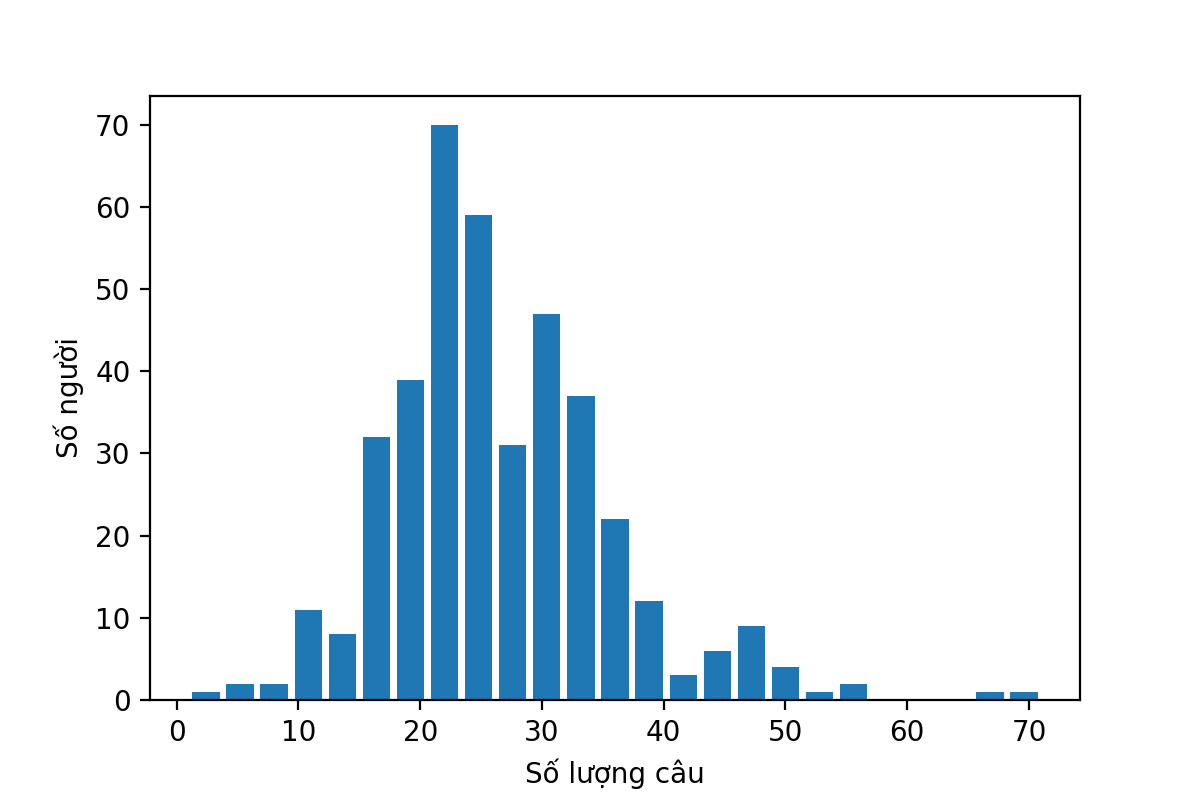
\includegraphics[width=0.8\textwidth]{images/zaloai.png}
  \caption{Biểu đồ phân phối số danh tính theo số câu nói của bộ dữ liệu ZaloAI.}
  \label{fig:zaloai}
\end{figure}

Với 8.7 giờ và 400 danh tính, bộ dữ liệu ZaloAI so với hơn 2,000 giờ và 7,000 danh tính trong bộ dữ liệu VoxCeleb là quá nhỏ bé. Để bổ sung thêm dữ liệu cho bài toán, tác giả sử dụng nguồn dữ liệu công khai nhận dạng tiếng nói tiếng Việt. Các bộ dữ liệu nhận dạng tiếng nói tiếng Việt bao gồm VLSP, INFORE, VIVOS và FPT. Trong đó, chỉ bộ dữ liệu VLSP và VIVOS có nhãn người nói. Đồ án tiến hành khảo sát các bộ dữ liệu VIVOS và VLSP để bổ sung dữ liệu cho bài toán xác minh người nói tiếng Việt.

VIVOS là tập giọng nói tiếng Việt phục vụ cho bài toán nhận dạng tiếng nói thu thập bởi phòng thí nghiệm khoa học máy tính AILAB từ trường Đại học Khoa học Tự nhiên - Đại học Quốc Gia TP.HCM \cite{VIVOS}. Tuy chủ đích của bộ dữ liệu là dành cho nhận dạng tiếng nói nhưng lại có nhãn danh tính cụ thể nên có thể sử dụng cho bài toán nhận dạng người nói. Tập huấn luyện VIVOS bao gồm 40 danh tính với trung bình 253.5 câu nói mỗi người. Tập kiểm thử có 19 danh tính không trùng với tập huấn luyện với trung bình 40 câu nói mỗi người. Chất lượng âm thanh của VIVOS rất tốt do điều kiện thu âm được kiểm soát nên không yêu cầu xử lý gì thêm.

Bộ dữ liệu VLSP \cite{VLSP} nằm trong chiến dịch đánh giá năm 2020 của Hiệp hội xử lý Ngôn ngữ và Tiếng nói tiếng Việt. Giống như VIVOS, VLSP được thu thập và thiết kế cho bài toán nhận diện giọng nói nhưng có nhãn danh tính cho các câu nói. Tổng số danh tính trong VLSP là $567$ người với trung bình $22.3$ câu mỗi người. Tuy nhiên, dữ liệu danh tính của bộ dữ liệu lại không được chuẩn xác và có nhiều vấn đề tương tự như bộ ZaloAI. Những vấn đề này được giải quyết bằng phương pháp mô tả trong phần \ref{noise-removal}.

Ngoài các bộ dữ liệu tương đối lớn được mô tả bên trên, đồ án còn thu thập thêm dữ liệu từ CommonVoice \cite{CommonVoice}. CommonVoice là dự án nguồn cung cứng cộng đồng bắt nguồn từ Mozilla để tạo các cơ sở dữ liệu miễn phí nhằm phát triển nhận dạng tiếng nói. Bộ dữ liệu tiếng Việt được xác thực đến từ CommonVoice gọi là CommonVoice-vi chỉ bao gồm 23 người và 253 câu nói. Với lượng dữ liệu ít ỏi và tính chất nhìn chung khác với các bộ dữ liệu còn lại. Trong hai tập kiểm tra, CommonVoice đóng vai trò làm bộ kiểm thử ngoài miền huấn luyện.

\subsection{Tổng quan quy trình}

Bộ dữ liệu phục vụ cho bài toán được xây dựng theo quy trình (Hình \ref{fig:data-cleaning}) bắt đầu với việc gộp  dữ liệu người nói từ nhiều nguồn khác nhau thành một bộ dữ liệu lớn để làm sạch. Quá trình làm sạch bao gồm ba bước: loại bỏ danh tính không hợp lệ, loại bỏ đoạn tiếng nói không hợp lệ và hợp nhất có cùng danh tính. Bộ dữ liệu đầu ra sau đó được tách thành tập huấn luyện và 2 tập kiểm thử. Chi tiết về làm sạch dữ liệu và bộ dữ liệu được trình bày trong các phần sau.

\begin{figure}[h]
  \centering
  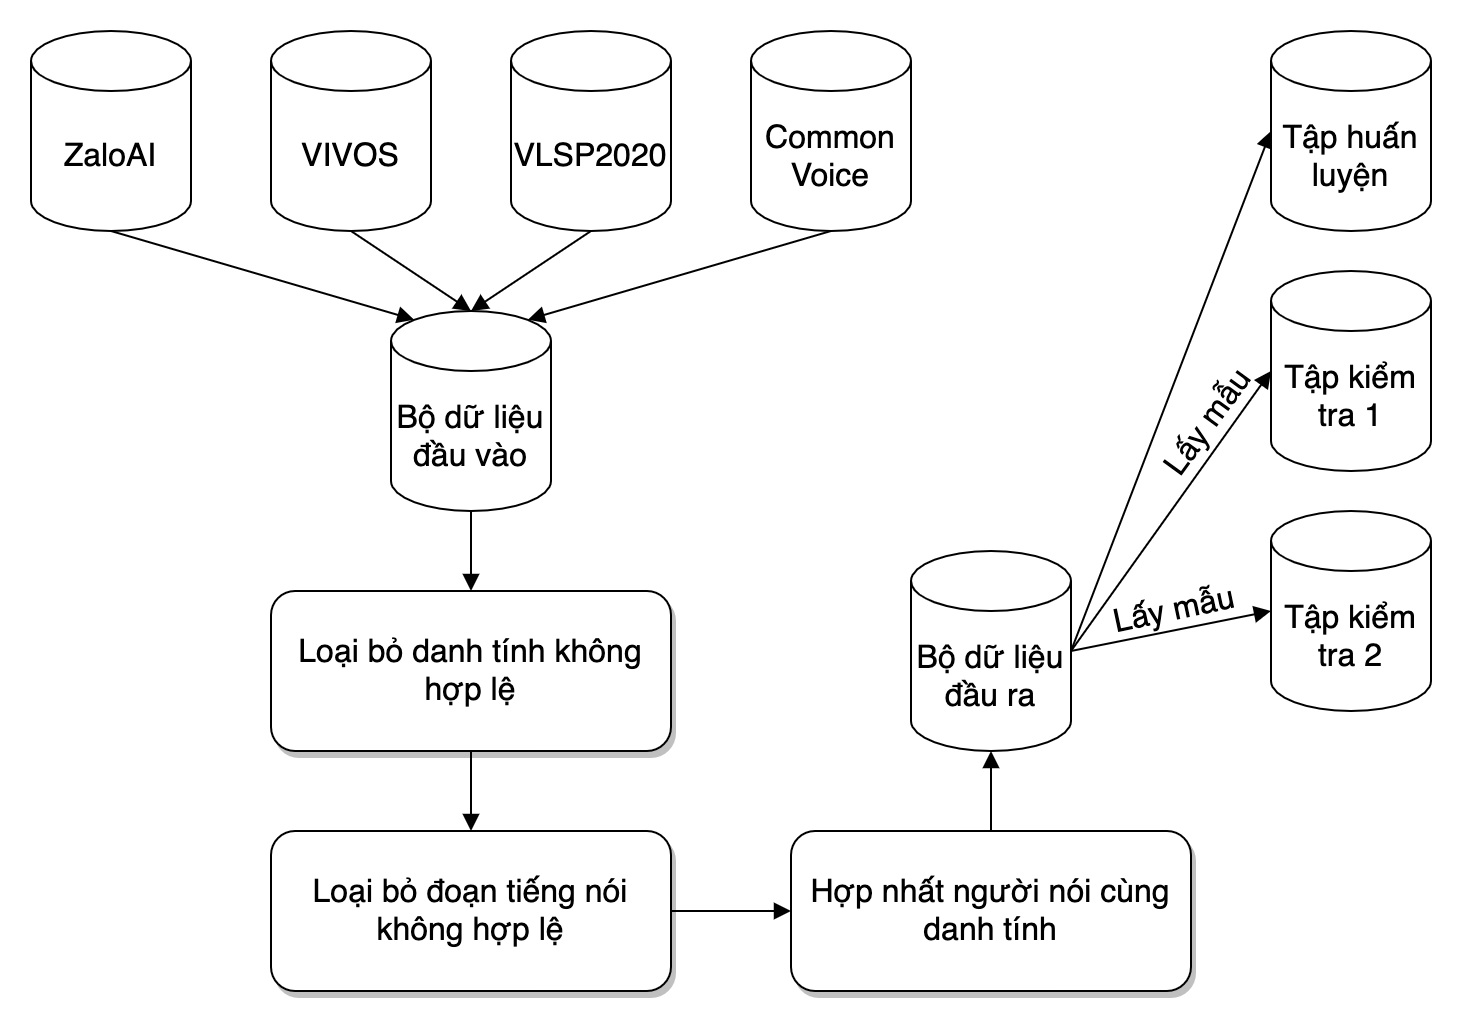
\includegraphics[width=0.9\textwidth]{images/data-process.png}
  \caption{Quy trình xây dựng bộ dữ liệu.}
  \label{fig:data-cleaning}
\end{figure}


\subsection{Làm sạch dữ liệu} \label{noise-removal}
Các bộ ZaloAI, VIVOS, VLSP cùng CommonVoice-vi có tổng cộng gần 1 nghìn danh tính và hơn 20 nghìn câu. Do vậy, việc kiểm tra dữ liệu rất khó khăn và tốn thời gian. Việc này còn trở nên khó khăn hơn khi đánh giá bằng tai người, ví dụ để phân biệt giọng của 2 người cùng là nam, giọng trầm miền bắc thì cần sự tập trung cao độ để tìm điểm khác biệt. Vì thế, đồ án phân tích ma trận tương đồng của các câu nói để tìm ra sự không nhất quán từ đó thu hẹp phạm vi kiểm tra.

Cho một tập biểu diễn $n$ đoạn âm thanh đầu vào $\bm{V} = \{\bm{v}_0, \bm{v}_1, ..., \bm{v}_{n-1}\}$, sử dụng độ tương đồng cô-sin, ma trận tương đồng cho các đoạn tiếng nói được tính theo Công thức \ref{eq:experiments1}. Ví dụ một ma trận tương đồng trong Hình \ref{fig:similarity-example}, đường chéo chính có giá trị tương đồng là 1 do so sánh mỗi câu với chính câu đó.

\begin{equation} \label{eq:experiments1}
  \bm{S}_{i,j} = cos(\bm{v}_i, \bm{v}_j) = \dfrac{\bm{v}_i \cdot \bm{v}_j}{\|\bm{v}_i\| \|\bm{v}_j\|}, 0 \leq i,j \le n
\end{equation}

\begin{figure}[h]
  \centering
  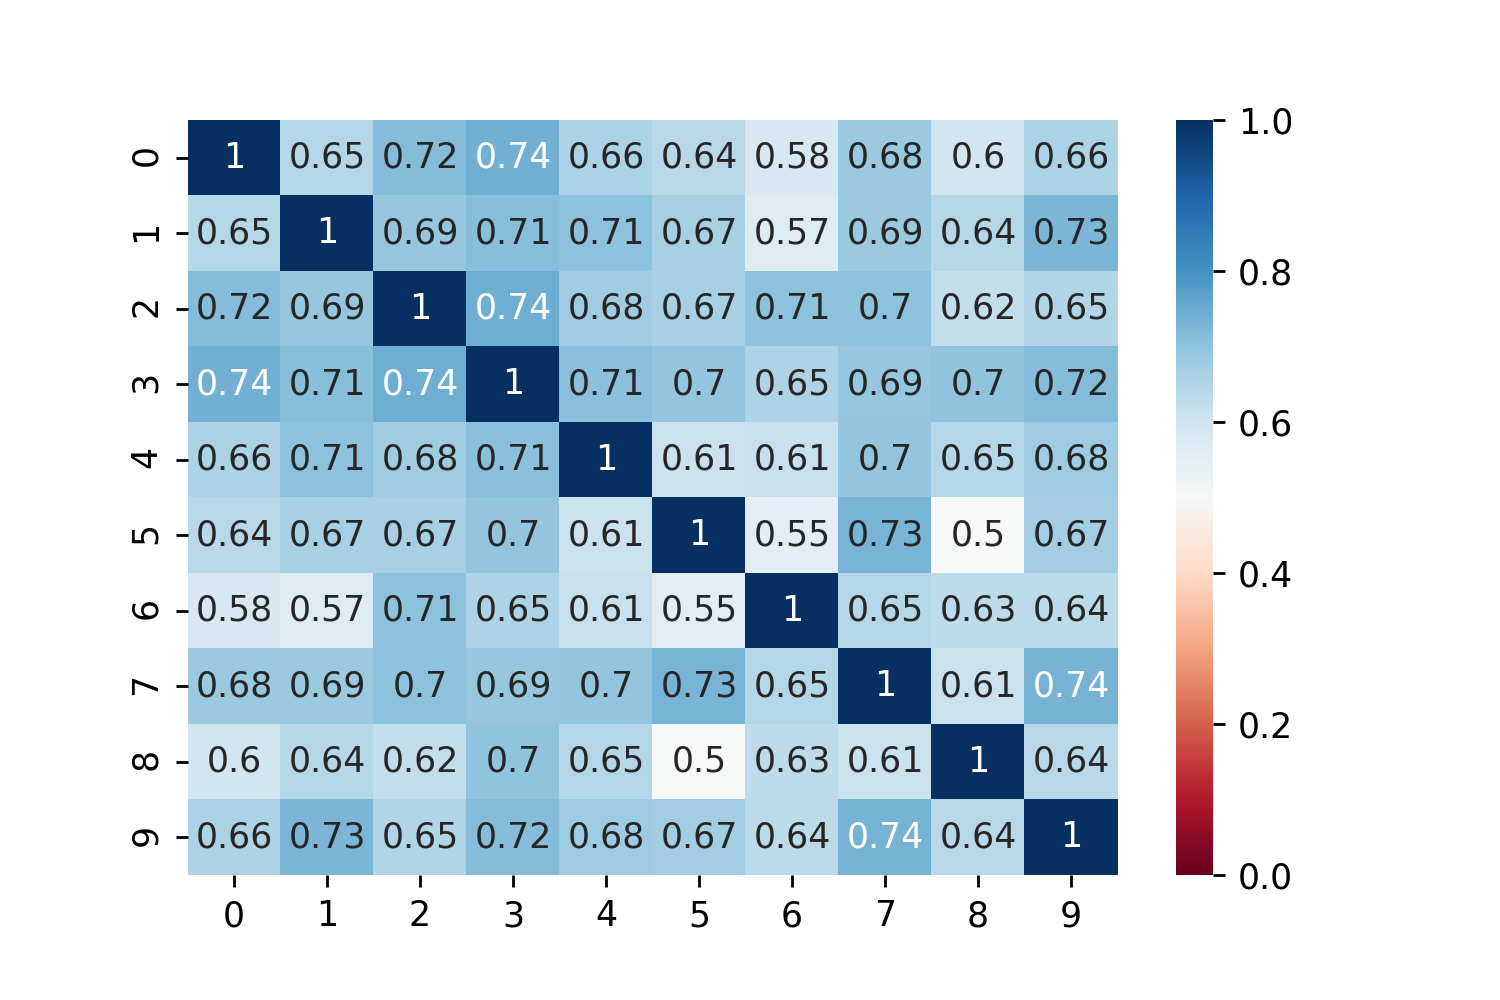
\includegraphics[width=0.9\textwidth]{images/similarity.png}
  \caption{Ma trận tương đồng cho một tập 10 đoạn âm thanh của một người.}
  \label{fig:similarity-example}
\end{figure}

Ma trận tương đồng được áp dụng khá rộng rãi, trong đó, phổ biến nhất là phân tích âm nhạc dựa trên nội dung \cite{silva2018fast}, phân tích văn bản \cite{hussain2010improved} và tin sinh \cite{bustamam2018implementation}. Các kĩ thuật được sử dụng chủ yếu là phân cụm và phân đoạn. Trong đồ án, tác giả sử dụng phân tích đơn thuần để tìm ra các người nói, câu nói có khả năng bị gán nhãn sai.

\subsubsection{Loại bỏ người nói không hợp lệ}
Việc loại bỏ một danh tính có thể do nhiều lý do: nhiều câu nói không thuộc về người đó, chất lượng âm thanh kém, môi trường xung quanh ồn ào, tệp âm thanh bị hư hại qua đường truyền hoặc thiết bị, ... Các nguyên nhân này dẫn đến việc chất giọng của danh tính không được đảm bảo gây bất lợi cho việc huấn luyện mô hình. Một số danh tính có số lượng câu có vấn đề lớn, làm sạch và loại bỏ từng câu bằng việc nghe rất tốn thời gian và công sức. Do vậy, việc loại bỏ hẳn những danh tính này là cần thiết. Khi nhìn vào ma trận tương đồng của một danh tính, có thể thấy được và loại bỏ những danh tính không hợp lệ. Ma trận tương đồng của một người hợp lệ và bị loại bỏ có thể được thấy trong Hình \ref*{fig:similarity-example} và Hình \ref*{fig:similarity-speaker-eer} tương ứng.

\begin{figure}[h]
  \centering
  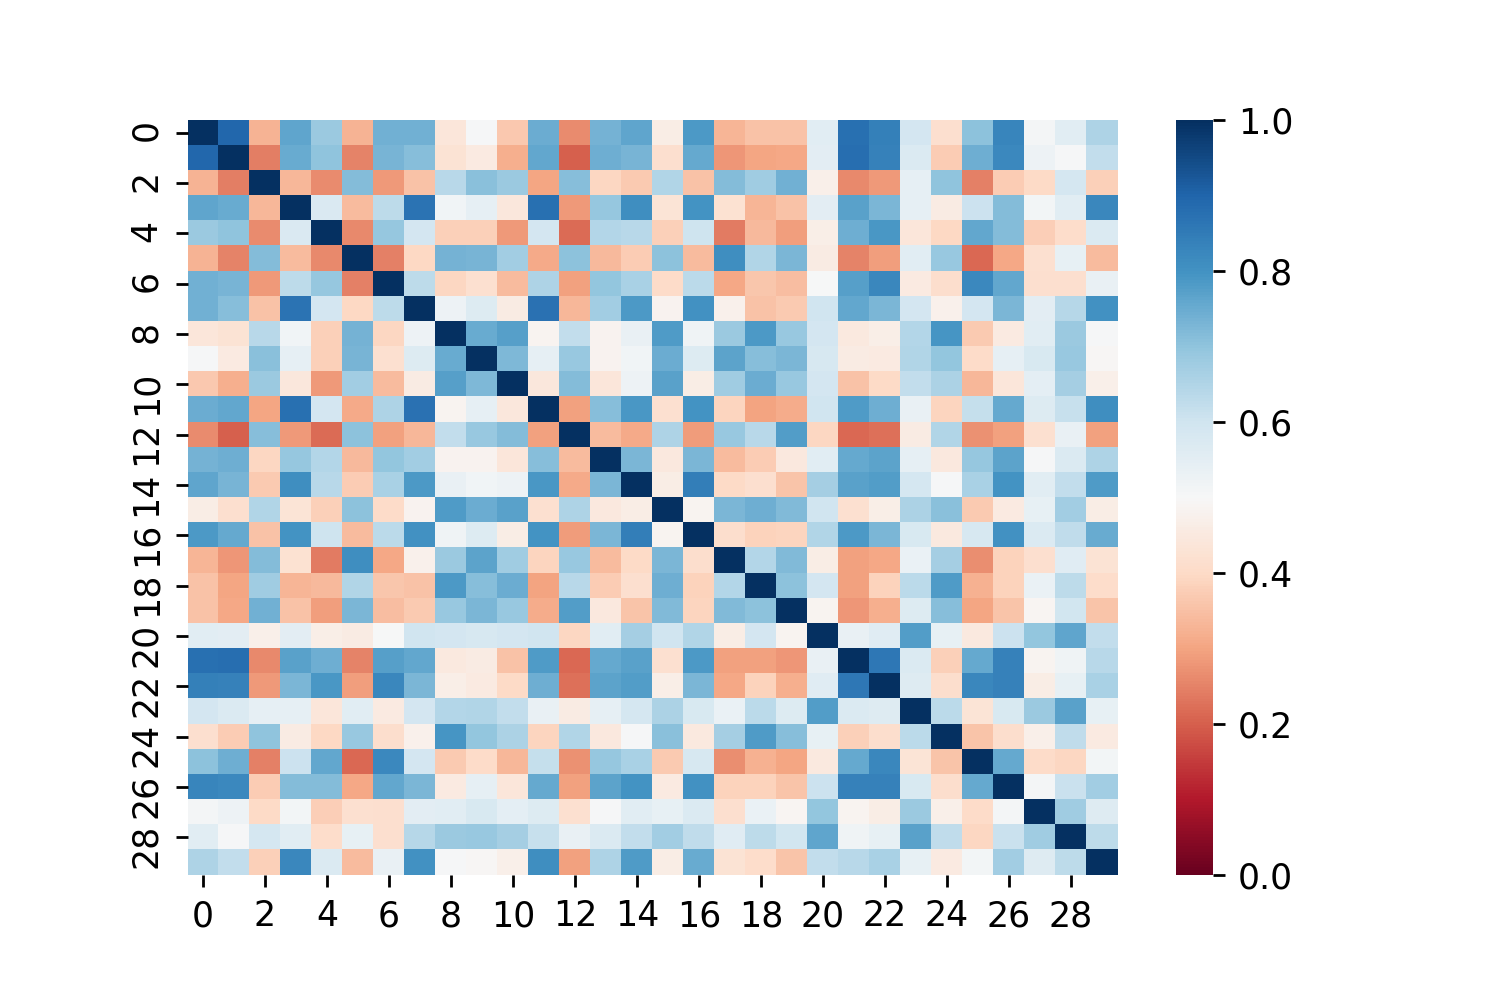
\includegraphics[width=0.9\textwidth]{images/similarity-spk-eer.png}
  \caption{Ma trận tương đồng của một danh tính bị loại bỏ.}
  \label{fig:similarity-speaker-eer}
\end{figure}

\subsubsection{Loại bỏ đoạn tiếng nói không hợp lệ}
Các đoạn tiếng nói không hợp lệ bao gồm sai nhãn danh tính, độ dài quá ngắn, tiếng ồn xung quanh quá lớn hay trong một đoạn có giọng của nhiều người khác nhau. Các đoạn này làm cho việc huấn luyện mô hình gặp khó khăn và giảm chất lượng của mô hình đầu ra. Lấy ma trận tương đồng của một người có câu nói không hợp lệ (Hình \ref{fig:similarity-utt-eer}) làm ví dụ, để lọc ra đoạn có chỉ số 6 khá đơn giản bằng cách lấy một ngưỡng thấp (ví dụ 0.3). Những câu có độ tương đồng so với những câu khác của một danh tính mà dưới ngưỡng này ta sẽ xem là không hợp lệ. Tuy nhiên, cách này không hợp lý với những câu như câu chỉ số 2 trong Hình \ref*{fig:similarity-utt-eer}, có điểm nằm trong khoảng 0.4 - 0.6. Tuy có điểm tương đồng khá cao nhưng những câu này cũng cần được kiểm tra. Những câu này có thể được tìm thấy bằng cách phát hiện ngoại lệ sử dụng khoảng trong tứ phân vị (Interquartile range) \cite{yang2019outlier}.

Với, Q1, Q3 lần lượt là tứ phân vị thứ nhất và thứ ba của tập điểm trung bình của các câu $a_i = \dfrac{1}{n} \sum_{j=0, j \neq i}^{n-1}\bm{S}_{i,j}$, dựa trên khoảng trong tứ phân vị, đoạn điểm tương đồng hợp lệ cho tập điểm $\bm{a}$ được tính theo hai Công thức \ref{eq:iqr1} và \ref{eq:iqr2}.

\begin{equation}\label{eq:iqr1}
  a_{min} = Q1 - 1.5 * IQR;\ a_{max} = Q3 + 1.5 * IQR
\end{equation}

\begin{equation} \label{eq:iqr2}
  IQR = Q3 - Q1
\end{equation}

Các câu có điểm trung bình $a_i$ nằm ngoài đoạn $[a_{min}, a_{max}]$ được đánh dấu và cần nghe lại để quyết định có loại bỏ hay không. 

\begin{figure}[h]
  \centering
  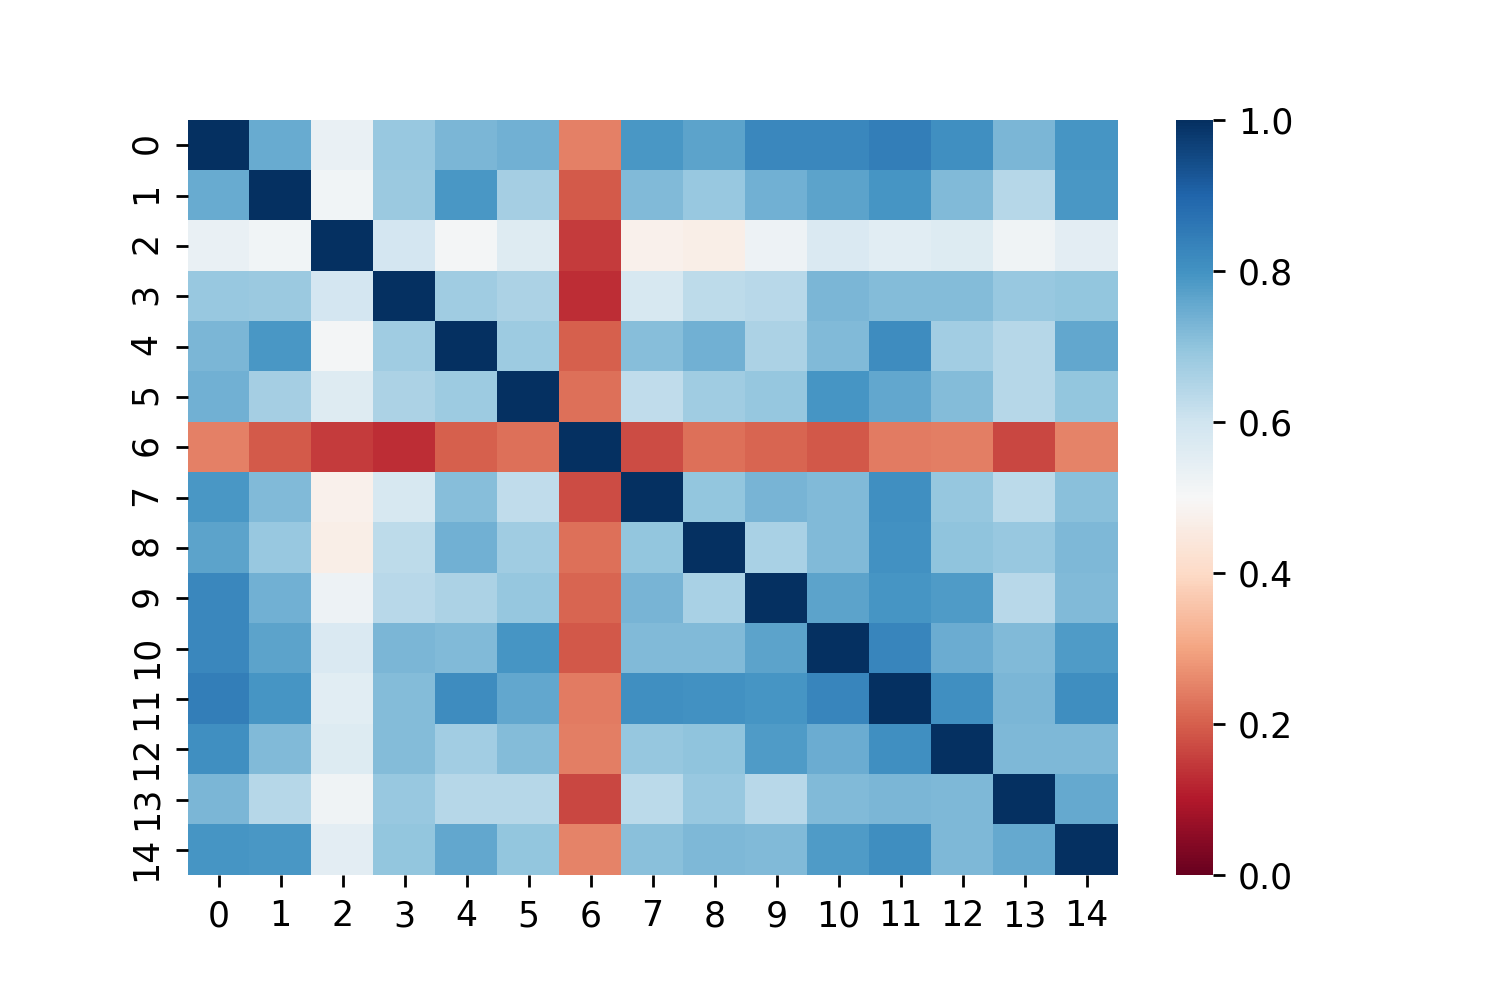
\includegraphics[width=0.9\textwidth]{images/similarity-utt-eer.png}
  \caption{Ma trận tương đồng của một danh tính có đoạn âm thanh không hợp lệ.}
  \label{fig:similarity-utt-eer}
\end{figure}

\subsubsection{Hợp nhất người nói có cùng danh tính}
Do các bộ dữ liệu được thu thập một cách độc lập, có khả năng người nói trong bộ dữ liệu này trùng với bộ kia. Hơn nữa, một người đã tồn tại trong cơ sở dữ liệu cũng có khả năng được yêu cầu thu lại. Các cặp người nói trùng danh tính có thể được tìm dựa vào ma trận tương đồng chéo. Từ Hình \ref*{sub@fig:similarity-cross-sub1} mô tả ma trận tương đồng của người nói 52-M-31 và 64-M-30, có thể thấy rõ đây là 2 người khác nhau do ma trận tương đồng chéo (phần màu đỏ) có điểm tương đồng rất thấp. Ngược lại, trong Hình \ref*{fig:similarity-cross-sub2}, 2 người có nhãn khác nhau là 64-M-30 và 636-M-30 thực chất là cùng một người với ma trận tương đồng chéo nằm trong ô màu đỏ. Có nhiều cặp câu điểm tương đồng cao (ô xanh đậm) nhưng không đạt tới $1.0$ như trên đường chéo chính do cơ bản có cùng nội dung nhưng khác biệt đến từ sự biến đổi nhất định trong quá trình xử lý. Các cặp người nói có giá trị trung bình của ma trận tương đồng chéo lớn hơn $0.7$ yêu cầu được nghe lại và ra quyết định để hợp nhất.

\begin{figure}
  \centering
  \begin{subfigure}{.5\textwidth}
    \centering
    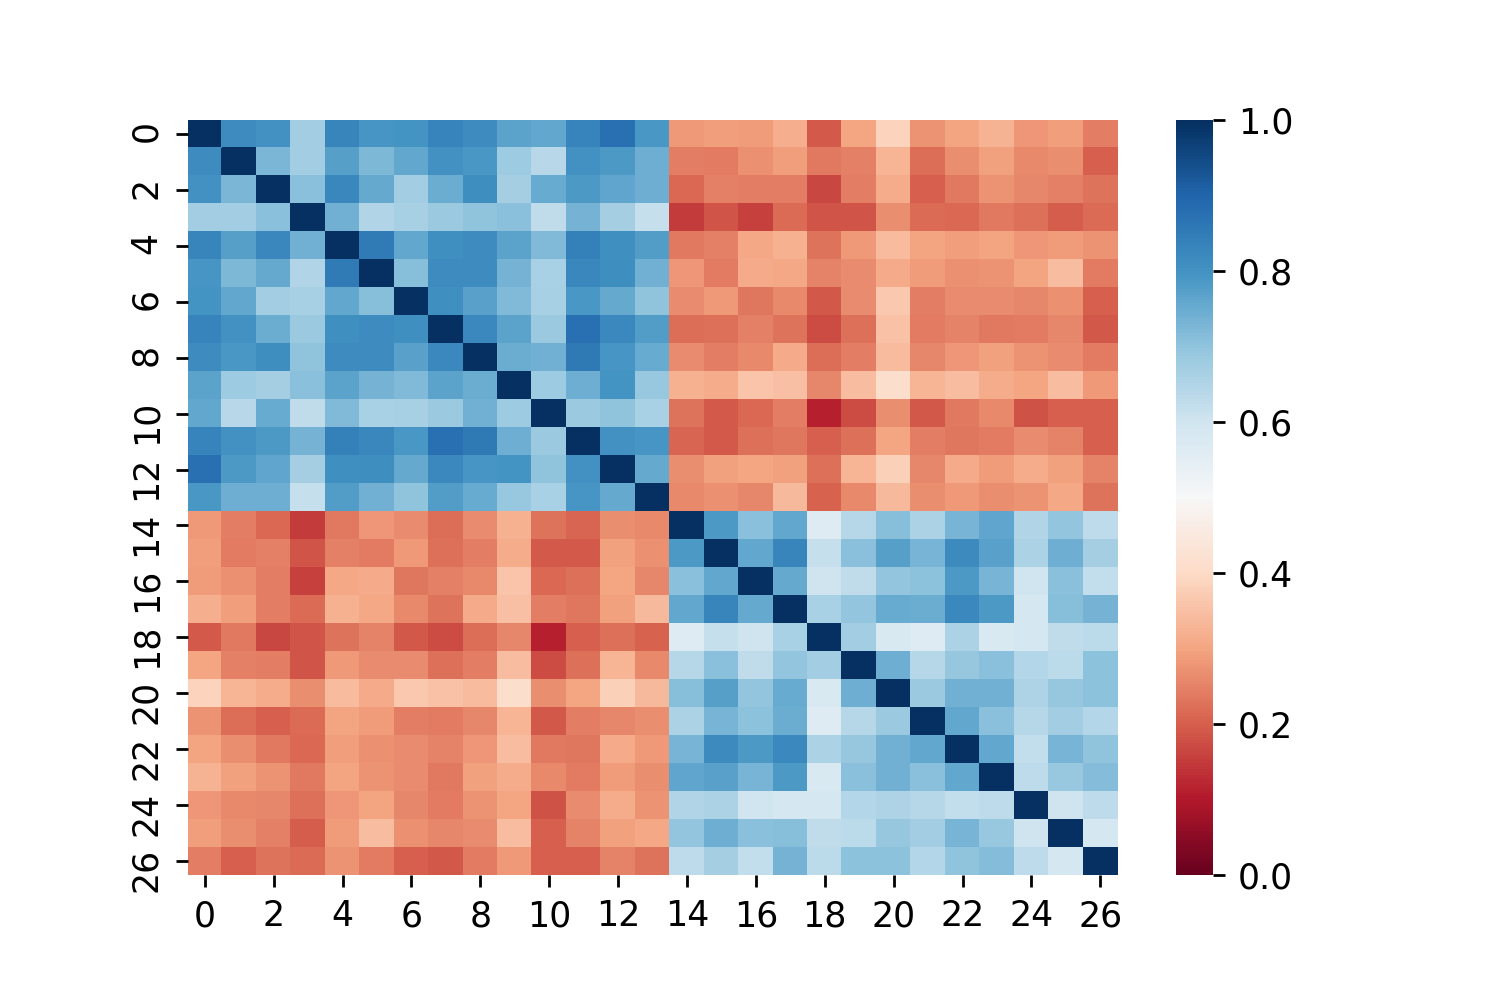
\includegraphics[width=\textwidth]{images/similarity-cross1.png}
    \caption{Ma trận tương đồng của 52-M-31 và 64-M-30.}
    \label{fig:similarity-cross-sub1}
  \end{subfigure}%
  \begin{subfigure}{.5\textwidth}
    \centering
    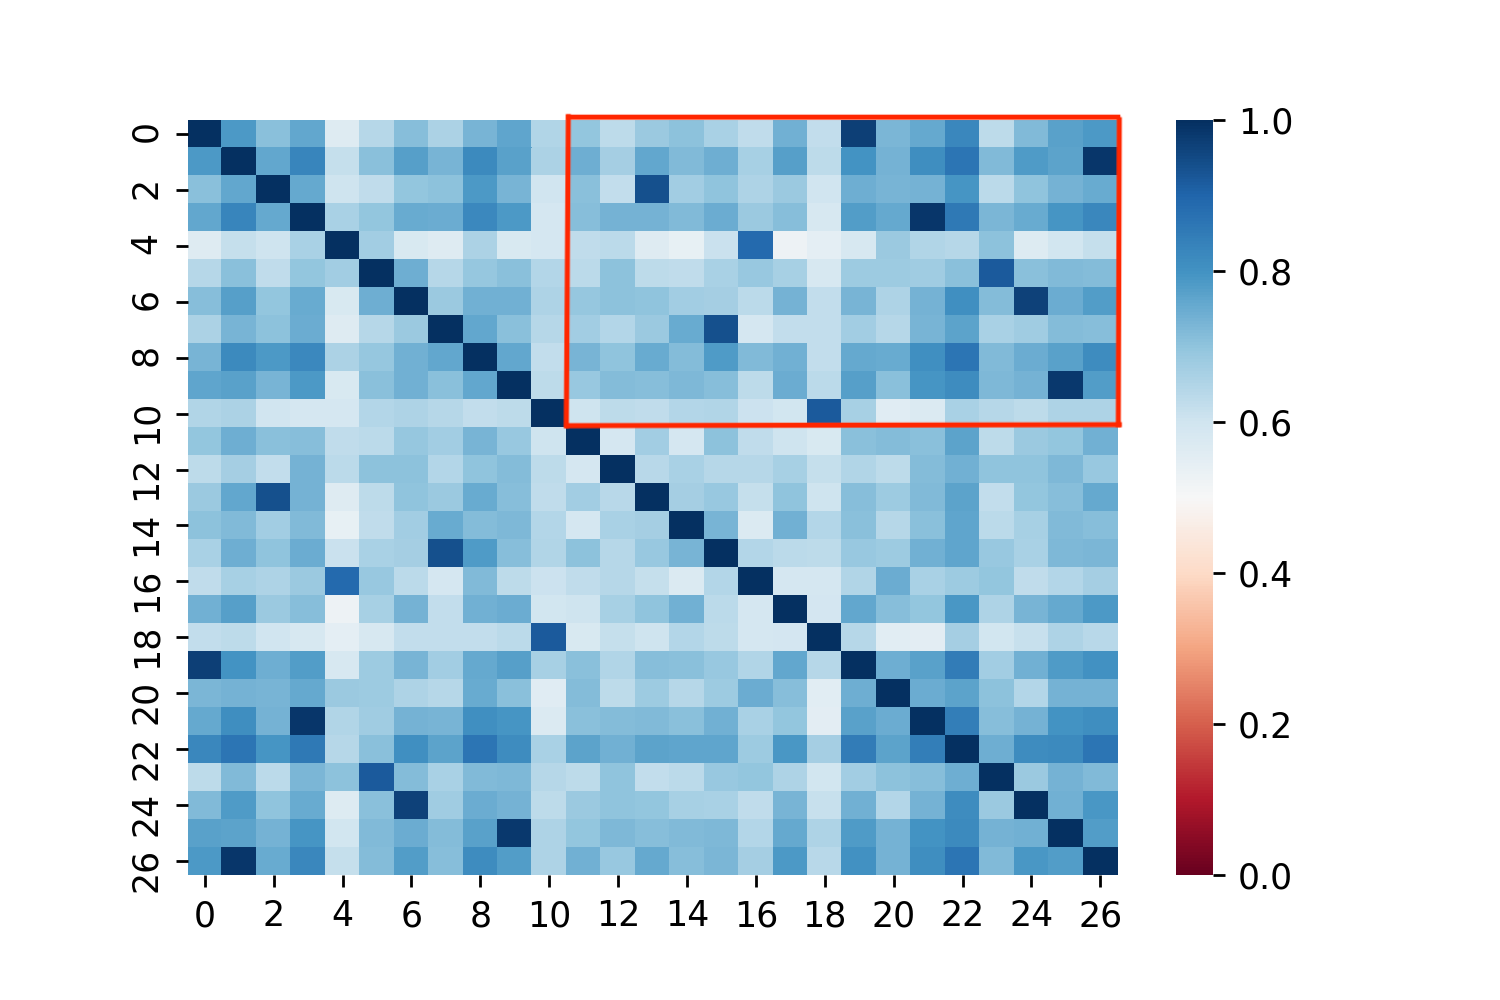
\includegraphics[width=\textwidth]{images/similarity-cross2.png}
    \caption{Ma trận tương đồng của 64-M-30 và 636-M-30.}
    \label{fig:similarity-cross-sub2}
  \end{subfigure}
  \caption{Ma trận tương đồng cho các cặp người nói khác nhau.}
  \label{fig:similarity-cross-sub2}
\end{figure}

% \subsubsection{Tổng kết cải thiện chất lượng dữ liệu}
% Bảng \ref*{tab:data-filtering} tổng kết thông tin sàng lọc dữ liệu. Số người nói bị loại bỏ chiếm 5.15\% tổng số người nói, số người nói được hợp nhất chiếm 6.67\% tổng số người nói, số câu nói bị loại bỏ chiếm 6.16\% tổng số câu. 

% \begin{table}[h]
%   \centering
%   \begin{tabular}{|l|r|r|r|}
%     \hline
%     \textbf{Bộ dữ liệu}& \textbf{Số danh tính loại bỏ} & \textbf{Số danh tính hợp nhất} & \textbf{Số câu loại bỏ} \\
%     \hline
%     ZaloAI  & 0   & 51  & 1,066 \\
%     VIVOS   & 0   & 0   & 2 \\
%     VLSP    & 65  & 33  & 549 \\
%     Tổng    & 65  & 84  & 1,617 \\
%     \hline
%   \end{tabular}
%   \caption{Thông số sàng lọc dữ liệu}
%   \label{tab:data-filtering}
% \end{table}


% Checked 
\subsection{Bộ dữ liệu VietSV}
Sau khi loại bỏ 65 danh tính không phù hợp, hợp nhất 84 người nói vào người nói khác có cùng danh tính và loại bỏ 1,617 các câu có vấn đề, bộ dữ liệu đã có chất lượng tương đối tốt. Tổng số lượng người nói là 1113, được phân thành 3 tập: tập huấn luyện (training set) gồm 1031 người nói, tập kiểm tra 1 (test set 1) và tập kiểm tra 2 (test set 2). Bộ dữ liệu gồm 3 tập này được đặt tên là VietSV \ref{tab:vietsv}.

\begin{table}[h]
  \centering
  \begin{tabular}{|l|r|r|}
    \hline
    \textbf{Tập dữ liệu} & \textbf{Số người nói} & \textbf{Số cặp câu}\\
    \hline
    Tập huấn luyện & 1031 & - \\
    Tập kiểm tra 1 & 59   & 48,148 \\
    Tập kiểm tra 2 & 23   & 12,192 \\
    \hline
  \end{tabular}
  \caption{Thông số sàng bộ dữ liệu VietSV}
  \label{tab:vietsv}
\end{table}

Tập kiểm tra 1 bao gồm 48,148 cặp đoạn tiếng nói từ 59 người nói với tổng số 1,626 đoạn tiếng nói. Trong đó, 20 người được lấy ngẫu nhiên trong bộ ZaloAI với điều kiện cân bằng giới tính nam - nữ, 19 người còn lại trong tập kiểm tra là tập kiểm thử (development set) của bộ dữ liệu VIVOS. Để tăng độ khó cho các tập kiểm tra, các cặp tiếng nói âm tính được lấy mẫu ngẫu nhiên từ người nói có cùng giới tính và vùng miền. Tập kiểm tra 2 (test set 2) bao gồm 12,192 cặp đoạn tiếng nói từ 23 người nói trong CommonVoice với tổng số 253 câu nói. Cách lấy mẫu của tập kiểm tra 2 cũng tương tự như tập kiểm tra 1. Tuy số lượng câu nói trong tập kiểm tra tương đối nhỏ, độ khó của tập này đến từ việc dữ liệu trong tập này có tính chất khác với tập huấn luyện.

Trong đồ án này, tập huấn luyện được trích ra một nhóm 20 người cân bằng giới tính để sử dụng làm tập kiểm thử (validation set). Trong các thử nghiệm trong phần \label{experiment}, đồ án sử dụng tập kiểm tra 1.

\section{Chuẩn bị thực nghiệm} \label{experiment}
\subsection{Môi trường thực nghiệm}
Để thực hiện huấn luyện các mô hình, tác giả sử dụng Google Colaboratory: Hệ điều hành Ubuntu 18.04, 2vCPU Intel Xeon 2.2 Ghz, RAM 25GB, GPU Tesla T4 15GB.

Các thực nghiệm trong mục tiếp theo đều được chạy trên cùng bộ thông số như sau:
\begin{itemize}
  \item Đặc trưng âm học: filter banks.
  \item Tăng cường dữ liệu: nhiễu MUSAN \cite{snyder2015musan}, tiếng vang \cite{ko2017study}.
  \item Mạng trích xuất đặc trưng: ResNet.
  \item Lớp tổng hợp: Tổng hợp thống kê tập trung.
  \item Batch size: 100.
\end{itemize}

\subsection{Độ đo đánh giá}
Trong phần thực nghiệm, tác giả sử dụng tỉ lệ lỗi bằng nhau (Equal Error Rate - EER) để đánh giá hiệu năng của các mô hình thực nghiệm. EER là điểm nằm cắt nhau giữa đường tỉ lệ chấp nhận giả (False Acceptance Rate - FAR, tỉ lệ mà người xâm nhập được coi là người dùng hợp lệ) và đường tỉ từ chối giả (False Rejection Rate - FRR, tỉ lệ mà người dùng hợp lệ bị từ chối) khi điều chỉnh ngưỡng (Hình \ref{fig:eer}). Mô hình nhận dạng người nói càng hiệu quả thì có EER càng nhỏ.

\begin{figure}[h]
  \centering
  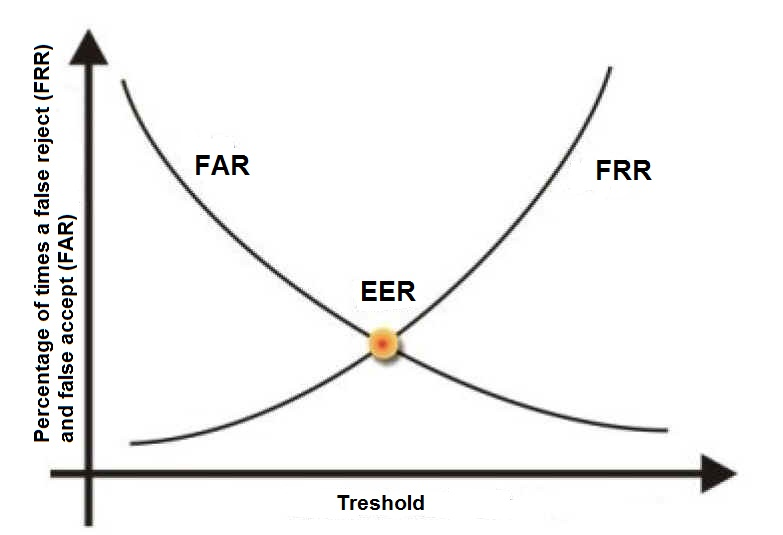
\includegraphics[width=0.6\textwidth]{images/eer.jpg}
  \caption{Mô tả EER \protect\footnotemark.}
  \label{fig:eer}
\end{figure}
\footnotetext{https://wentzwu.com/2019/05/05/which-is-more-important-accuracy-or-acceptability/}

Hệ thống tính điểm cho một cặp câu bằng việc tính độ tương đồng cô-sin của biểu diễn của 2 đoạn tiếng nói. Hai câu nói của cùng một người nói được coi là hợp lệ; hai câu nói từ 2 người nói khác nhau được coi là câu nói không hợp lệ. Với một ngưỡng cho trước, nếu cặp điểm câu nói hợp lệ dưới ngưỡng này (độ tương đồng thấp), câu nói đó được tính vào tỉ lệ từ chối giả. Ngược lại, nếu một cặp câu nói không hợp lệ có điểm nằm trên ngưỡng (tỉ lệ tương đồng cao), câu nói được tính vào tỉ lệ chấp nhận giả.

\subsection{Cài đặt thực nghiệm}
Để cài đặt thực nghiệm, tác giả sử dụng ngôn ngữ lập trình Python kết hợp với thư viện PyTorch phiên bản 1.7.1. PyTorch là thư mã nguồn mở của Facebook được xây dựng trên ngôn ngữ lập trình Lua. PyTorch cho phép người dùng xây dựng, tuỳ biến mô hình ở cả cấp cao và cấp thấp với thiết kế trực quan.

Trong đồ án, tác giả sử dụng mã nguồn mô hình trong \cite{chung2020defence} và cài đặt các phần liên quan tới huấn luyện và các phương pháp đề xuất. Ngoài ra, tác giả cũng sử dụng mã nguồn mô hình ECAPA \cite{thienpondt2020cross} và cài đặt các phần huấn luyện để so sánh với phương án đề xuất.

\section{Kết quả thực nghiệm và đánh giá}

Tác giả thực hiện nhiều trường hợp thực nghiệm khác nhau với mục tiêu huấn luyện mô hình nhận dạng người nói một cách hiệu quả trên tiếng Việt. Thực nghiệm 1 đánh giá hiệu quả của việc làm sạch dữ liệu. Thực nghiệm 2 khảo sát học chuyển tiếp so với các cách huấn luyện khác nhau. Thực nghiệm 3 đánh giá hiệu quả trong việc khử nhiễu âm thanh tín hiệu giọng nói. Thực nghiệm 4 so sánh mô hình khi sử dụng phương thức tối ưu Adam và SGD. Thực nghiệm 5 kiểm tra tính hiệu quả của hàm mất mát AMP-cos và AMP-arc với các giá trị hệ số phạt khác nhau. Thực nghiệm 6 so sánh mô hình đề xuất với mô hình ECAPA sử dụng học chuyển tiếp trong \cite{thienpondt2020cross}.

\subsection{Thực nghiệm 1: Làm sạch dữ liệu}
Bảng \ref*{tab:experiment-clean} mô tả kết quả thực nghiệm với dữ liệu ban đầu và dữ liệu đã được làm sạch như đã trình bày trong phần \ref*{noise-removal}. Như có thể thấy, kết quả huấn luyện trên tập đã sàng lọc cải thiện 0.93\% EER so với dữ liệu gốc. Do vậy, các thực nghiệm về sau sẽ sử dụng bộ dữ liệu đã qua sàng lọc.

\begin{table}[h]
  \centering
  \begin{tabular}{|l|r|}
    \hline
    \textbf{Dữ liệu}& \textbf{EER trên tập kiểm tra}\\
    \hline
    Bộ dữ liệu ban đầu & 8.532\% \\
    \textbf{Bộ dữ liệu VietSV} & \textbf{7.602\%} \\
    \hline
  \end{tabular}
  \caption{EER trên tập kiểm tra với dữ liệu trước và sau khi cải thiện chất lượng}
  \label{tab:experiment-clean}
\end{table}

\subsection{Thực nghiệm 2: Học chuyển tiếp}
Trong thực nghiệm này, tác giả tiến hành khảo sát các phương thức huấn luyện mô hình. Bảng \ref{tab:experiment-training} mô tả kết quả với các trường hợp khác nhau bao gồm: mô hình huấn luyện sẵn \cite{heo2020clova}, huấn luyện từ đầu trên dữ liệu tiếng Anh và tiếng Việt, huấn luyện từ đầu chỉ trên VietSV, học chuyển tiếp trên VietSV. 

Do số người nói trong bộ dữ liệu VietSV ít hơn hẳn so với người nói tiếng Anh trong bộ dữ liệu VoxCeleb, huấn luyện không tập trung đủ để tìm ra các đặc trưng hữu ích để phân biệt người nói tiếng Việt, dẫn đến mô hình huấn luyện từ đầu kết hợp hai bộ dữ liệu đạt kết quả tệ hơn. Mô hình cơ sở (mô tả trong phần \ref{baseline}) huấn luyện từ đầu trên VietSV đạt kết quả 7.602\% EER. Học chuyển tiếp bằng riêng dữ liệu tiếng Việt cho kết quả tốt hơn so với huấn luyện từ đầu bằng trên VietSV hoặc kết hợp VoxCeleb với EER 5.890\%. Kết quả cho thấy các đặc trưng người nói trong tiếng Anh góp phần cải thiện mô hình tiếng Việt. Các thử nghiệm phía sau sử dụng phương pháp học chuyển tiếp.

\begin{table}[h]
  \centering
  \begin{tabular}{|l|l|r|}
    \hline
    \textbf{Phương pháp huấn luyện} & \textbf{Dữ liệu huấn luyện} & \textbf{EER trên tập kiểm tra}\\
    \hline
    Mô hình cơ sở & VoxCeleb & 14.954\% \\
    Mô hình cơ sở & VoxCeleb + VietSV & 8.499\% \\
    Mô hình cơ sở & VietSV & 7.602\% \\
    \textbf{Học chuyển tiếp} & \textbf{VietSV} & \textbf{5.890\%} \\
    \hline
  \end{tabular}
  \caption{EER trên tập kiểm tra với các phương pháp huấn luyện và dữ liệu khác nhau}
  \label{tab:experiment-training}
\end{table}

\subsection{Thực nghiệm 3: Khử tạp âm trong tín hiệu tiếng nói}
Do chỉ có VIVOS là được thu thập từ phòng thu âm, tín hiệu tiếng nói trong tập dữ liệu còn chứa nhiều tạp âm, ví dụ nhạc nền, tiếng ồn nhỏ xung quanh, âm thanh đường phố xe cộ. Các nhiễu tạp âm có khả năng cản trở mô hình học được giọng cần học từ dữ liệu. Do đó, tác giả sử dụng dữ liệu khử tạp âm dùng mô hình do bộ phận nghiên cứu trí tuệ nhân tạo tại Facebook phát triển \cite{defossez2020real} và đánh giá hiệu quả trong thực nghiệm này. Bảng \ref*{tab:experiment-denoising} cho thấy việc khử tạp âm có hiệu quả cao với 0.444\% EER cải thiện trên tập kiểm tra. Do vậy, trong các thực nghiệm tiếp theo, các mô hình được huấn luyện trên dữ liệu đã lọc tạp âm.

\begin{table}[h]
  \centering
  \begin{tabular}{|l|r|}
    \hline
    \textbf{Dữ liệu huấn luyện}& \textbf{EER trên tập kiểm tra}\\
    \hline
    Chứa tạp âm & 5.890\% \\
    \textbf{Khử tạp âm} & \textbf{5.446\%} \\
    \hline
  \end{tabular}
  \caption{EER trên tập kiểm tra của mô hình huấn luyện với dữ liệu còn nhiễu âm thanh và đã khử tạp âm}
  \label{tab:experiment-denoising}
\end{table}

\subsection{Thực nghiệm 4: Phương pháp tối ưu SGD}
Bảng \ref{tab:experiment-optimizer} cung cấp kết quả 2 mô hình huấn luyện bằng phương pháp tối ưu Adam và SGD. Kết quả huấn luyện với SGD cải thiện tới 1.907\% so với mô hình huấn luyện với Adam. Thật vậy, khi quan sát giá trị của hàm mất mát trên tập huấn luyện trong hình \ref{fig:sgd-vs-adam1}, sự hội tụ của Adam khá nhất quán, thậm chí có phần tốt hơn SGD. Tuy nhiên, trong phần \ref{fig:sgd-vs-adam2}, kết quả EER trên tập kiểm thử của Adam rất không nhất quán ngay từ những vòng lặp đầu, trong khi SGD hội tụ rất tốt trên tập kiểm thử và không có dấu hiệu học quá khớp. Điều này chứng minh khả năng khái quát hoá vượt trội của SGD so với Adam cho bài toán.

\begin{table}[h]
  \centering
  \begin{tabular}{|l|r|}
    \hline
    \textbf{Phương pháp tối ưu}& \textbf{EER trên tập kiểm tra}\\
    \hline
    Adam & 5.446\% \\
    \textbf{SGD} & \textbf{3.539\%} \\
    \hline
  \end{tabular}
  \caption{EER trên tập kiểm tra của mô hình huấn luyện với Adam và SGD}
  \label{tab:experiment-optimizer}
\end{table}

\begin{figure}[h]
  \centering
  \begin{subfigure}{.5\textwidth}
    \centering
    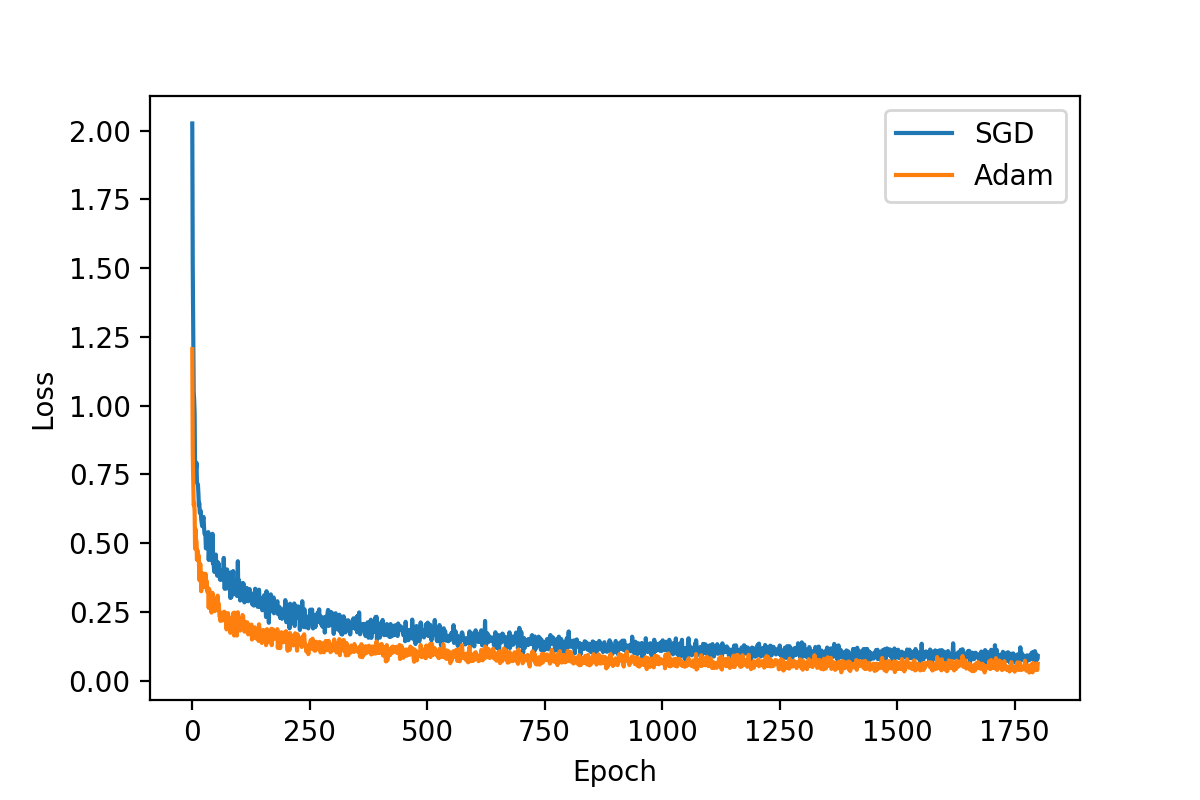
\includegraphics[width=\textwidth]{images/loss.png}
    \caption{Giá trị hàm mất mát trên tập huấn luyện.}
    \label{fig:sgd-vs-adam1}
  \end{subfigure}%
  \begin{subfigure}{.5\textwidth}
    \centering
    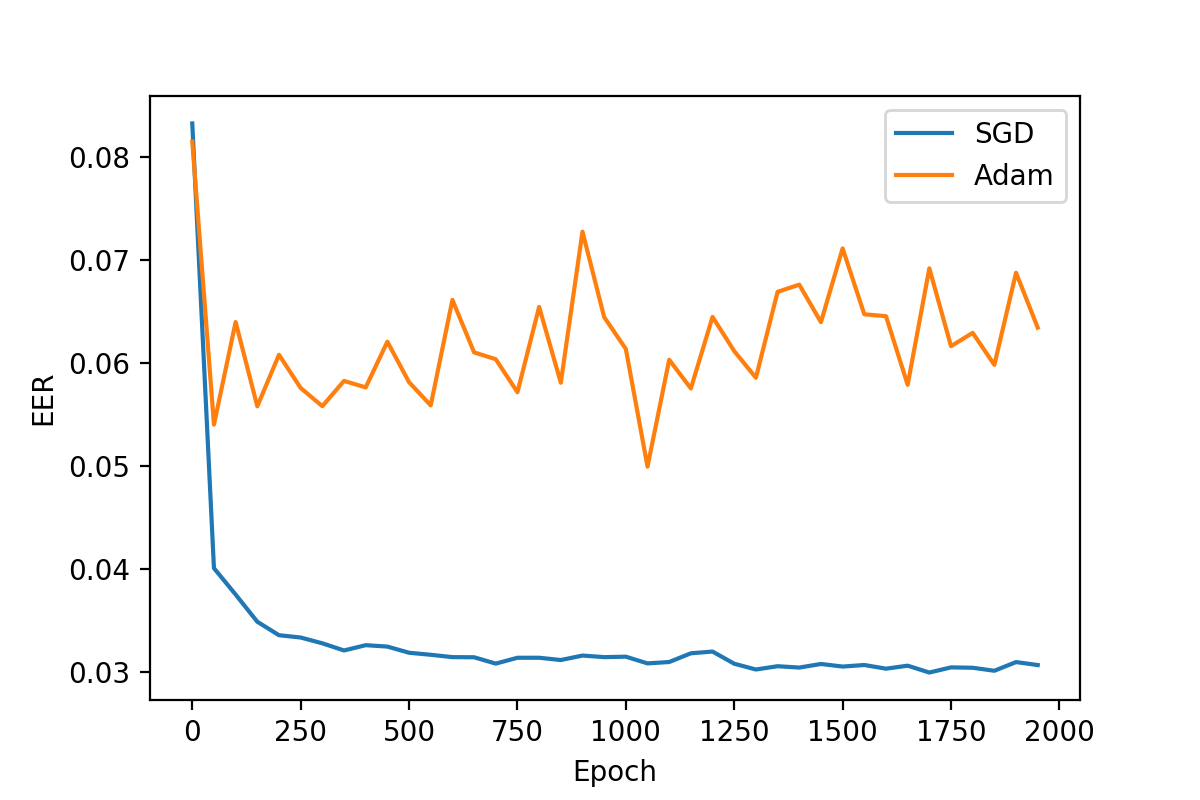
\includegraphics[width=\textwidth]{images/eer.png}
    \caption{EER trên tập kiẻm thử.}
    \label{fig:sgd-vs-adam2}
  \end{subfigure}
  \caption{So sánh giá trị mất mát và EER của mô hình huấn luyện với SGD và Adam qua các vòng lặp.}
  \label{fig:sgd-vs-adam}
\end{figure}

Các mô hình trong thực nghiệm 5 sử dụng phương pháp tối ưu SGD.

\subsection{Thực nghiệm 5: Hàm mất mát AMP}
Bảng \ref{tab:experiment-loss} mô tả kết quả thử nghiệm khi sử dụng hai phiên bản phạt biên khác nhau AMP-cos, AMP-arc của hàm AP. Nhìn chung, việc sử dụng hàm AMP có hiệu quả tích cực khi huấn luyện mô hình. Hai hàm AMP-cos và AMP-arc với hệ số phạt lần lượt là $m=0.4$ và $m=0.2$ cho kết quả 3.211\% và 3.115\% tương ứng. Với các giá trị khác nhau của $m$, AMP luôn tốt hơn so với hàm AP thông thường. Trong AMP-arc, với $m$ lớn hơn 0.2, kết quả có xu hướng tệ đi khi tăng giá trị của $m$ do hiện tượng quá khớp.

\begin{table}[h]
  \centering
  \begin{tabular}{|l|r|r|}
    \hline
    \textbf{Hàm mất mát}& \textbf{$m$} & \textbf{EER trên tập kiểm tra}\\
    \hline
    AP & 0.0 &3.539\% \\
    AMP-cos & 0.1 & 3.319\% \\ 
    AMP-cos & 0.2 & 3.269\% \\
    AMP-cos & 0.3& 3.232\% \\
    AMP-cos & 0.4 & 3.211\%\\
    AMP-cos & 0.5 & 3.331\%\\
    AMP-arc & 0.1 & 3.240\% \\ 
    \textbf{AMP-arc} & \textbf{0.2} & \textbf{3.115\%} \\
    AMP-arc & 0.3 & 3.194\% \\
    AMP-arc & 0.4 & 3.298\%\\
    AMP-arc & 0.5 & 3.352\%\\
    \hline
  \end{tabular}
  \caption{EER trên tập kiểm tra của mô hình huấn luyện với hàm mất mát AP, AMP-cos và AMP-arc với các giá trị phạt khác nhau}
  \label{tab:experiment-loss}
\end{table}

\begin{figure}[h]
  \centering
  \begin{subfigure}{.5\textwidth}
    \centering
    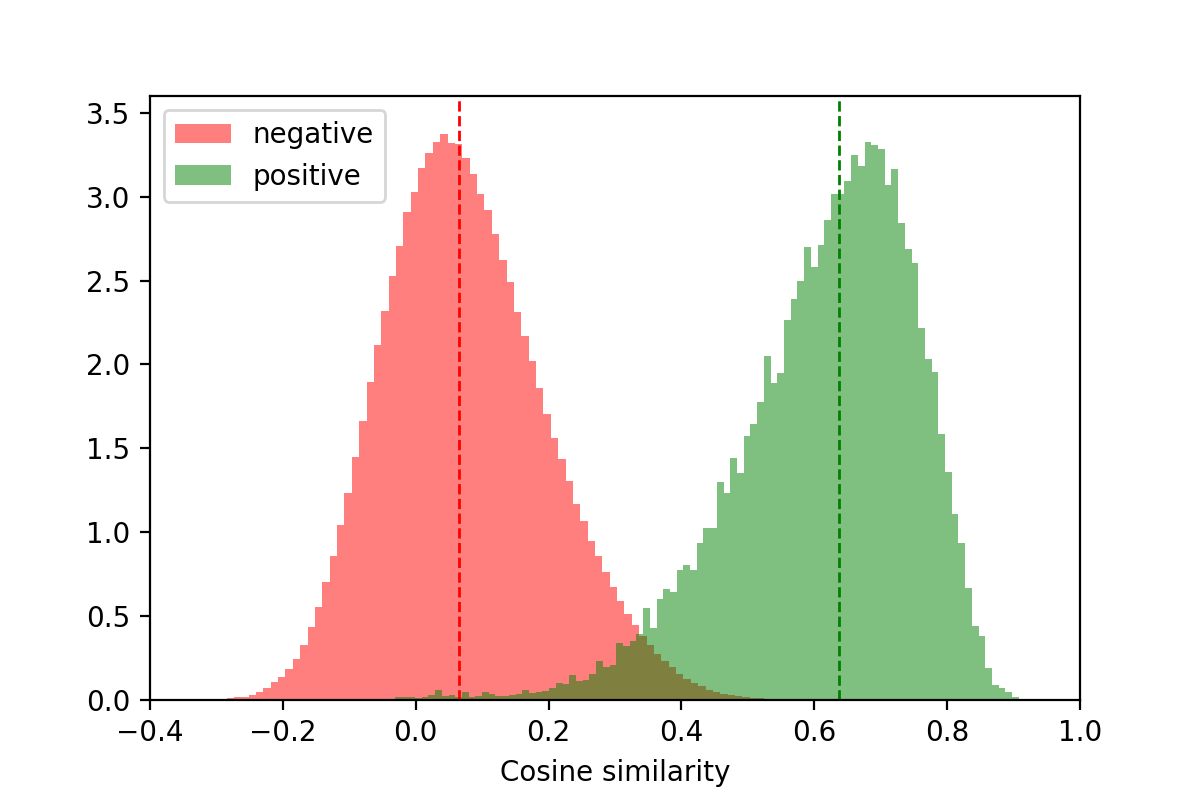
\includegraphics[width=\textwidth]{images/distribution.png}
    \caption{Mô hình huấn luyện với AP}
    \label{fig:score-distribution1}
  \end{subfigure}%
  \begin{subfigure}{.5\textwidth}
    \centering
    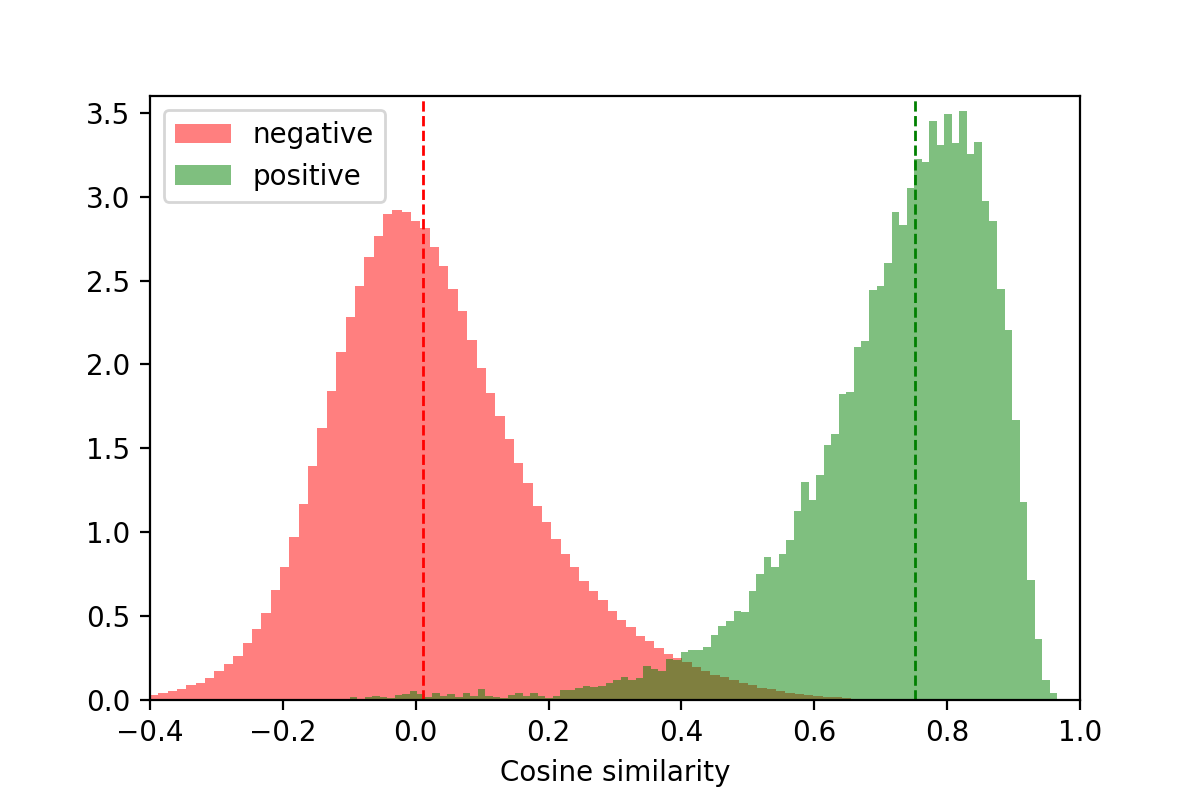
\includegraphics[width=\textwidth]{images/distribution-margin.png}
    \caption{Mô hình huấn luyện với AMP-arc (m=0.2)}
    \label{fig:score-distribution2}
  \end{subfigure}
  \caption{Phân bố điểm tương đồng của các cặp câu dương tính và âm tính. Các đường nét đứt mô tả giá trị trung bình điểm trương đồng.}
  \label{fig:score-distribution}
\end{figure}

Để hiễu rõ hơn về tính phân loại của biểu diễn người nói, phân bố điểm tương đồng cho các cặp câu dương tính và âm tính được thể hiện trong Hình \ref*{fig:score-distribution}. Hình \ref*{fig:score-distribution1} thể hiện phân bố điểm đoán bởi mô hình huấn luyện với hàm AP, Hình \ref*{fig:score-distribution2} thể hiện phân bố điểm đoán bởi mô hình huấn luyện với hàm AMP-arc (m=0.2). Hiệu quả của tính nhận dạng được quyết định bởi phần chồng lên nhau ở giữa của hai phân bố dương tính và âm tính. Với hàm AMP-arc, phần đuôi chồng nhau của hai phân bố nhỏ hơn và phần thân của hai phân bố nghiêng về phía ngược lại đối với phần chồng nhau. Ngoài ra, khoảng cách của điểm trung bình dương và âm tính được tăng lên gần 0.2 so với hàm AP, từ đó tăng tính phân loại.

\subsection{Thực nghiệm 6: So sánh mô hình đề xuất và ECAPA}
Bảng \ref{tab:experiment-other} mô tả kết quả giữa mô hình đề xuất và mô hình ECAPA đề xuất trong \cite{thienpondt2020cross}. Mô hình ECAPA sử dụng học chuyển tiếp dùng hàm mất mát HPM có mục tiêu tương tự đồ án: phát triển mô hình xác minh người nói cho ngôn ngữ ít dữ liệu trong khuôn khổ cuộc thi SdSV 2020. 

\begin{table}[h]
  \centering
  \begin{tabular}{|l|r|}
    \hline
    \textbf{Phương pháp tối ưu}& \textbf{EER trên tập kiểm tra}\\
    \hline
    \textbf{AMP-arc} & \textbf{3.115\%} \\
    ECAPA-Adam & 4.017\% \\
    ECAPA-SGD & 4.299\% \\
    \hline
  \end{tabular}
  \caption{EER của phương pháp đề xuất và phương pháp \cite{thienpondt2020cross}}
  \label{tab:experiment-other}
\end{table}


\subsection{Tổng kết kết quả thực nghiệm}

Qua 6 phần thực nghiệm trình bày ở trên, có thể thấy rằng việc xử lý dữ liệu bao gồm làm sạch dữ liệu giúp cải thiện mô hình đầu ra. Phương pháp kết hợp sử dụng học chuyển tiếp, khử tạp âm tín hiệu giọng nói, SGD, và AMP-arc (m=0.2) đạt 3.115\% EER cải thiện 4.487\% so với mô hình cơ sở với 7.602\% EER trên tập kiểm tra. 

\begin{figure}[h]
  \centering
  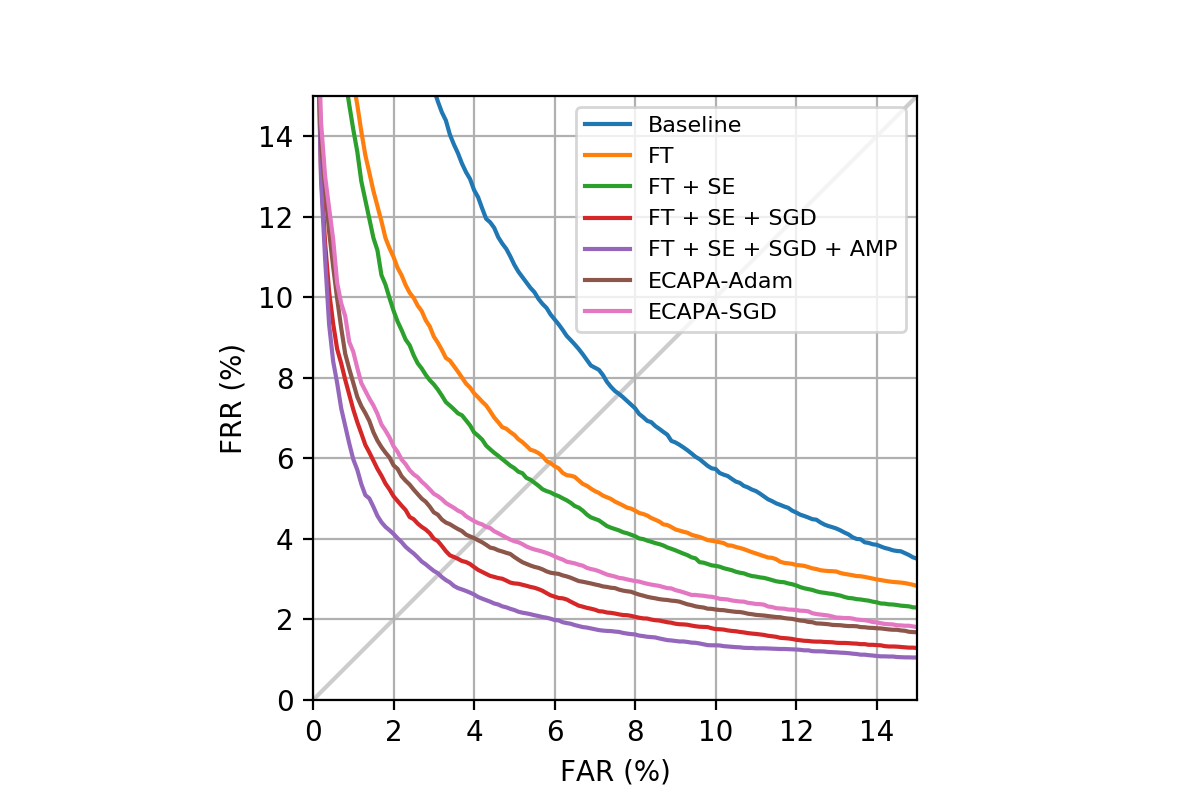
\includegraphics[width=0.9\textwidth]{images/det.png}
  \caption{Đường cong DET với mô hình cơ sở và các cải tiến. Đường EER $x=y$ màu xám. FT: Học chuyển tiếp, SE: speech enhancement - khử tạp âm.}
  \label{fig:det}
\end{figure}

Đường cong đánh đánh đổi lỗi phát hiện (detection error tradeoff - DET) cho mô hình cơ sở và các mô hình cải tiến được mô tả trong Hình \ref*{fig:det}. Các điểm trên một đường đại diện cho một cặp FAR và FRR tại một ngưỡng nhất định. Có thể thấy rằng mô hình đề xuất tốt hơn mô hình cơ sở trên mọi điểm. Giả sử do nhu cầu mà một hệ thống muốn tỉ lệ chấp nhận nhầm kẻ xấu FAR là 2\%, mô hình đề xuất cho tỉ lệ từ chối nhầm FRR tương đối thấp xấp xỉ 4\% trong khi mô hình cơ sở cho kết quả cao tới khoảng 17-18\% FRR.